% ===================== d_project.tex : the project from zero, condensed hard (chapters 1 to 18) =====================
\section{The whole project in five minutes}\label{ch:whole}

When a river overflows or heavy rain falls, people need to know where the water will be in the next few hours. A \term{physics simulator} can work this out but is slow (the dataset makers report days for one large flood). We teach a \term{neural network} to do the same job quickly. We show it the last few depth maps (each a map of the water depth in every little square of land), plus the rain and the ground height, and ask it to draw the \emph{next} map.

We used the public dataset \term{FloodCastBench}: four floods re-created in a simulator from real ground heights, land maps and satellite rain, in Australia, the UK, Pakistan and Mozambique. The network learns from Australia and Pakistan. The UK and Mozambique stay hidden until the final test, to see whether it works on a place it has never met.

\textbf{The key question.} In 30 minutes the water in most places hardly changes, so even ``copy the last map'' is a very good forecast. A model is only worth using if it beats simple guesses. The score is called \term{skill}: 0 means no better than copying and 1 means perfect.

\begin{enumerate}
\item \textbf{Model A} (CNN-LSTM, Colab) beat copying in 3 of 4 tests, and at first we were happy.
\item The \textbf{trend forecast} (take the last map and keep most of the last 30-minute change going, one fitted number, no network) scored 0.91 to 0.99, while Model A scored only 0.15 to 0.35 where it beat copying. In late Australia Model A was \emph{worse} than copying (skill $-1.449$).
\item \textbf{Model B} starts from the trend and learns a small correction. It matched the trend but did not beat it, because only 1\% to 9\% of the error of copying is left after the trend.
\item A laptop study (about 310 training runs, up to 2.5 hours ahead) found a linear formula scoring 0.79 to 0.82 (after a bug fix, \xref{Chapter}{ch:bug}) against 0.81 to 0.87 for the best networks. The LSTM memory did not help at equal training.
\item On top we built a \textbf{capsule network} that rates the flooding, \textbf{written rules} that check it (\emph{NeuroSymbolic AI}) and \textbf{Grad-CAM} heat maps (\emph{explainable AI}).
\end{enumerate}
The lesson: \textbf{always compare a model with simple forecasts before you trust it.}

\begin{table}[!htbp]
\centering\small
\caption{The two parts of the project. Their numbers must never be compared with each other.}
\begin{tabularx}{\linewidth}{|>{\bfseries}p{2.2cm}|Y|Y|}
\hline
\rowcolor{black!12} & \hd{Part 1: Colab notebook} & \hd{Part 2: laptop study}\\ \hline
Where it ran & Google Colab, GPU & One laptop, CPU\\ \hline
How far ahead & One map, 30 minutes & Five maps in a row, up to 2.5 hours\\ \hline
Input size & Whole maps (learns on 64 $\times$ 64 tiles) & Patches of 128 $\times$ 128 squares\\ \hline
Models and runs & Model A, Model B, trend, capsule, rules, Grad-CAM. One run each & CNN-LSTM, local CNN, ConvLSTMs, simple baselines. About 310 runs\\ \hline
\end{tabularx}
\end{table}

\fig{whole_system.png}{0.55}{Everything we built. The forecaster is Chapters 4 to 6 and 10, the capsule network and rules Chapter 15, Grad-CAM (dashed arrows) Chapter 16.}

% =========================================================== CHAPTER 2
\section{Floods, forecasts and the long title}\label{ch:why}

A \term{forecast} is a careful guess about the future. The simulator is detailed but slow, a trained network answers in seconds. The title decodes as: \textbf{CNN} (convolutional neural network, looks at pictures by sliding a small window, \xref{Chapter}{ch:cnn}), \textbf{LSTM} (long short-term memory, reads things in order and remembers, \xref{Chapter}{ch:lstm}), \textbf{spatiotemporal} (space and time) and \textbf{flood evolution} (how a flood grows and changes). So: \emph{use a network that sees pictures and remembers the past to forecast how flood water spreads in space as time passes.} It is a careful test of how much a CNN-LSTM adds over simple guesses, not a ready warning system, because the floods are simulated and the models learned to imitate the simulator.

% =========================================================== CHAPTER 3
\section{A picture is just a grid of numbers}\label{ch:grid}

A flood map is a \term{grid} of small squares, each holding one number: the water depth in metres (0.0 is dry). In Australia and the UK a square is \textbf{30 m} wide, in Pakistan and Mozambique \textbf{480 m} (16 times wider). The Australia map has 1073 $\times$ 1073 squares. We \textbf{never mix the two sizes}: one model for each.

For every square we also know the ground height, the rain and the land cover, like clear sheets stacked on one another. Each sheet is a \term{channel}. The model uses three: water depth, rain and a version of the ground height. Depth is stored every 5 minutes but rain only every 30, so we keep \textbf{one map every 30 minutes}, like a flipbook (the 10-day Australia flood becomes 481 maps). Depth is in metres, rain in mm per hour, and errors in centimetres.

% =========================================================== CHAPTER 4
\section{What is a neural network, and how does it learn?}\label{ch:nn}

A programmer normally writes rules, which is nearly impossible for water. A \term{neural network} is given many \emph{examples} and finds the rules itself: it \textbf{guesses, sees how wrong it was, and adjusts}. It is built from \term{neurons}. A neuron multiplies each input by its own \term{weight}, adds the results and applies a simple rule, \term{ReLU}: if the number is negative make it zero, otherwise leave it. ReLU adds the bend, without which many layers would be no better than one weighted sum. Many neurons side by side form a \term{layer}. The weights plus one bias per neuron are the \term{parameters}. Our main model has \textbf{62,833}.

\begin{figure}[!htbp]
\centering
\begin{tikzpicture}[>=Stealth,every node/.style={font=\small},scale=0.62,transform shape]
\node[circle,draw,minimum size=8mm,fill=mist] (x1) at (0,1.0) {2};
\node[circle,draw,minimum size=8mm,fill=mist] (x2) at (0,-0.4) {3};
\node[circle,draw,minimum size=15mm,fill=teal!12,align=center] (s) at (4.2,0.3) {add\\up};
\node[draw,rounded corners=2pt,minimum height=8mm,fill=amber!15,align=center] (r) at (7.6,0.3) {ReLU rule:\\negative $\to$ 0};
\node[circle,draw,minimum size=8mm,fill=mist] (o) at (10.3,0.3) {0};
\draw[->,thick] (x1) -- node[above,sloped] {weight 0.5} (s);
\draw[->,thick] (x2) -- node[below,sloped] {weight $-1$} (s);
\draw[->,thick] (s) -- node[above] {$-2$} (r);
\draw[->,thick] (r) -- (o);
\node[font=\footnotesize] at (4.2,-1.0) {$2\times0.5 + 3\times(-1) = -2$};
\end{tikzpicture}
\caption{One neuron with made-up numbers. The sum $-2$ is negative, so ReLU turns it into 0.}
\end{figure}

\paragraph{The learning loop.} Weights start random. Then the network repeats: \textbf{guess}, \textbf{measure} how wrong (the loss), \textbf{nudge} every weight a little. The \term{loss} is the \term{mean squared error}: square each mistake and average (squaring stops $-0.1$ and $+0.1$ cancelling and punishes big mistakes more). To know which way to nudge, the network uses the \term{gradient}, the slope of the mistake: like standing on a foggy hill, feeling which way the ground slopes and stepping downhill. The step size is the \term{learning rate}, the method that decides each step is the \term{optimiser}. \term{Adam} is a popular optimiser that adapts its step size, and we used it throughout with learning rate 0.001. The network nudges after a small group of examples, a \term{batch} (16 in Colab, 1 on the laptop). One trip through all training examples is an \term{epoch} (we call it a pass).

\paragraph{Overfitting and early stopping.} A network can memorise its practice examples and fail on anything new. This is \term{overfitting}. We split each flood in time order: training (first 70\%, learned from), validation (15\%, checked during training) and test (last 15\%, used only at the end). A never-seen flood is an even harder exam. The sign of overfitting is practice error falling while validation error rises, and \term{early stopping} stops when validation stops improving and keeps the best version (used in Part 1). We meet a real case in \xref{Chapter}{ch:res1}.

Models are written in \term{Python} with \term{TensorFlow} and \term{Keras}. A \term{GPU} does the many tiny calculations much faster than a \term{CPU}. Part 1 ran on a Colab GPU and Part 2 on one laptop CPU.

% =========================================================== CHAPTER 5
\section{Teaching a network to look at maps: the CNN}\label{ch:cnn}

A \term{convolutional neural network} (\term{CNN}) uses a small window called a \term{filter} (or \term{kernel}), commonly $3\times3$. We lay it over one spot, multiply the 9 numbers under it by 9 weights and add them: one number saying ``how much does this spot look like my pattern?'' Then we slide it one step (the \term{stride} is 1) until the map is covered, which gives a \term{feature map}. Adding a border of zeros (\term{padding}) keeps the map the same size. The \textbf{same filter is used everywhere}, so the parameter count stays small.

\begin{figure}[!htbp]
\centering
\begin{tikzpicture}[x=4mm,y=4mm,every node/.style={font=\small}]
\foreach \i in {1,...,5}{\foreach \j in {1,...,5}{\draw[black!45,fill=mist] (\i,\j) rectangle ++(1,1);}}
\draw[brick,very thick,fill=brick!15,fill opacity=0.6] (1,3) rectangle (4,6);
\draw[brick,very thick,dashed] (2,3) rectangle (5,6);
\node at (3.5,0.2) {map ($5\times5$)};
\draw[->,thick] (7.4,4.5) -- node[above,font=\footnotesize] {one number} node[below,font=\footnotesize] {per spot} (10.3,4.5);
\foreach \i in {1,...,3}{\foreach \j in {1,...,3}{\draw[black!45,fill=teal!10] (\i+11,\j+1) rectangle ++(1,1);}}
\draw[brick,very thick,fill=brick!30] (12,4) rectangle ++(1,1);
\draw[brick,very thick,dashed] (13,4) rectangle ++(1,1);
\node at (14.2,0.9) {new map ($3\times3$, no padding)};
\node[align=left,font=\footnotesize,text width=5.5cm] at (24,4) {The red window reads 9 squares and gives 1 number. The dashed window is the next step.};
\end{tikzpicture}
\caption{A filter slides over the map. Every spot gets one number.}
\end{figure}

One filter finds one pattern, so a layer uses many (for example 16), giving 16 feature maps that are the 16 \emph{channels} the next layer reads. A second convolution layer combines the simple patterns of the first (edges, slopes) into bigger ones such as a river bend, and each square sees a larger area. After each filter we apply ReLU. (Pooling is not used.) \textbf{Real count:} the first layer has 16 filters of $3\times3$ reading 3 channels, so $3\times3\times3=27$ weights plus 1 bias is 28 per filter and $16\times28=\mathbf{448}$ parameters. The second reads 16 channels: $3\times3\times16+1=145$ per filter and $16\times145=\mathbf{2{,}320}$.

% =========================================================== CHAPTER 6
\section{Teaching a network to remember: LSTM and ConvLSTM}\label{ch:lstm}

One flood map cannot tell you whether the water is rising, you need the map before it. An \term{LSTM} (\emph{long short-term memory}) reads one step at a time and keeps a memory, like a student with a notebook who at each step does three things: \textbf{forget} (erase what no longer matters), \textbf{write} (add what is useful) and \textbf{read} (look in the notebook to answer). Small dials called \term{gates} (forget, input, output) do these jobs, and the network learns how far to turn each. A normal LSTM keeps its memory as a short list of numbers. Ours must say something about \emph{each place}, so we use a \term{ConvLSTM}: its memory is a map and its gates use sliding filters like the CNN, so each square is updated using its neighbours too.

\begin{figure}[!htbp]
\centering
\begin{tikzpicture}[every node/.style={font=\small},scale=0.55,transform shape]
\foreach \i/\l in {0/{3 steps ago},3.2/{2 steps ago},6.4/{1 step ago},9.6/{now}}{
  \draw[fill=blue!15,draw=black!60] (\i,3) rectangle ++(1.4,1.0);
  \node at (\i+0.7,4.3) {\l};
  \draw[->,thick] (\i+0.7,3) -- (\i+0.7,2.25);
  \draw[fill=amber!25,rounded corners=2pt] (\i-0.2,1.2) rectangle ++(1.8,1.05);
  \node[align=center,font=\footnotesize] at (\i+0.7,1.72) {memory\\map};
}
\foreach \i in {0,3.2,6.4}{\draw[->,thick] (\i+1.6,1.72) -- (\i+3.0,1.72);}
\draw[->,thick] (10.3,1.2) -- (10.3,0.5) node[below,align=center,font=\small] {the next map (the forecast)};
\end{tikzpicture}
\caption{A ConvLSTM reads the maps in order and updates a memory that is itself a map.}
\end{figure}

Our ConvLSTM has 32 filters, and 55,424 of the 62,833 parameters live here. The big question of the project is: \textbf{does the memory actually help, or is a simpler method just as good?}

% =========================================================== CHAPTER 7
\section{The data: four floods}\label{ch:data}

\term{FloodCastBench} (Xu and co-authors, \emph{Scientific Data}, 2025) re-created four real floods in a physics simulator using real \textbf{ground height} (FABDEM), \textbf{land cover} and satellite \textbf{rain} (GPM-IMERG). Depth is given every 5 minutes, rain every 30. The maps are \textbf{simulated}, so our network learns to imitate the simulator, not real flooding.

\begin{table}[!htbp]
\centering\small
\caption{The four floods. ``Maps'' is the number of depth maps we keep, one every 30 minutes.}
\begin{tabularx}{\linewidth}{|>{\bfseries}l|Y|l|l|l|l|Y|}
\hline
\rowcolor{black!12} \hd{Flood} & \hd{Dates} & \hd{Square} & \hd{Map size} & \hd{Length} & \hd{Maps} & \hd{Our role}\\ \hline
Australia & 20 Feb to 2 Mar 2022 & 30 m & 1073 $\times$ 1073 & 10 days & 481 & Training\\ \hline
UK & 4 to 7 Dec 2015 & 30 m & 170 $\times$ 275 & 3 days & 145 & Never-seen test\\ \hline
Pakistan & 18 to 31 Aug 2022 & 480 m & 810 $\times$ 441 & 14 days & 673 & Training\\ \hline
Mozambique & 14 to 20 Mar 2019 & 480 m & 151 $\times$ 138 & 6 days & 289 & Never-seen test\\ \hline
\end{tabularx}
\end{table}

Australia and the UK also come at 60 m (used by the laptop study), made by resizing the 30 m results. Two pairs: learn from \textbf{Australia}, test on the \textbf{UK}, and learn from \textbf{Pakistan}, test on \textbf{Mozambique}.

\textbf{Getting the data ready.} (1) One map every 30 minutes. (2) One common grid: two independent checks (rivers of the land cover map and valleys of the ground height map against the water) agreed within about one square, then small squares were averaged into big ones. (3) Rain timing: rain file $j$ holds the rain in the 30 minutes \emph{after} depth map $j$, and on rainy steps the measured rise was 0.494 to 0.502 times the file value in all four floods, as expected for half an hour. (4) Three rain settings: \textbf{causal} (only past rain), \textbf{hybrid} (the original input, with up to 30 minutes of rain not yet fallen) and \textbf{forced} (the next five rain maps also given). (5) Local ground height: the height of a square minus the average around it (15 $\times$ 15 in Colab, the 128 $\times$ 128 patch on the laptop), because water flows by height differences. (6) \term{Tiles} (patches) of 64 $\times$ 64 in Colab and 128 $\times$ 128 on the laptop, because a million squares is too much in one piece. A trained network can then run on a whole map.

% =========================================================== CHAPTER 8
\section{The task and how we keep score}\label{ch:score}

\textbf{Part 1:} four depth maps 30 minutes apart plus rain and local height in, \textbf{one} map 30 minutes later out. \textbf{Part 2:} five maps in, the next five out (up to 2.5 hours) in one go.

\textbf{The simple forecasts we compare with.} \emph{Copy the last map} (persistence, skill 0 by definition), the \emph{trend forecast}, a \emph{linear model} of the depth history (fitted weighted sum), a \emph{lookup table} (average answer for each pair of current depth and last change) and a \emph{per-pixel MLP} (a tiny network looking at one square). The last three are Part 2 only. With $d_t$ the depth now and $d_{t-1}$ 30 minutes ago,
\[ \text{trend forecast} = \max\bigl(0,\; d_t + \beta\,(d_t - d_{t-1})\bigr). \]
Take the depth now, add a fraction $\beta$ of the last change, never go below zero. $\beta$ is fitted by least squares on the training part of the training flood only: \textbf{0.921} for 30 m and \textbf{0.948} for 480 m, a little below 1 so the change is continued but slightly slowed.

\textbf{The skill score.} Error is the average of squared mistakes over all squares, and
\[ \text{skill} = 1 - \frac{\text{error of the forecast}}{\text{error of copying the last map}}. \]
Skill 1 is perfect, 0 is no better than copying, below 0 is worse, and 0.9 removes 90\% of copying's error.

\textbf{Worked example.} Five squares: depth 30 minutes ago 0, 0.1, 0.4, 0.8, 1.0, now 0, 0.2, 0.5, 1.0, 1.0, what really happens 0, 0.3, 0.6, 1.2, 1.0. \emph{Copying} has mistakes 0, 0.1, 0.1, 0.2, 0 and squares adding to \textbf{0.06}. The \emph{trend} with $\beta=0.9$ gives 0, 0.29, 0.59, 1.18, 1.0, mistakes 0, 0.01, 0.01, 0.02, 0, squares adding to \textbf{0.0006}, so skill $=1-0.0006/0.06=0.99$. A \emph{bad model} giving 0, 0.5, 0.8, 1.1, 1.1 has squares adding to 0.10 and skill $\approx-0.67$, worse than copying (as Model A in late Australia, $-1.449$).

\fig{how_we_score.png}{0.45}{The skill score scale. \textbf{Say this:} 0 is copying the last map, 1 is perfect, negative is worse than copying.}

\textbf{Typical error in cm} (root mean square error) for copying the last map over the whole map: \textbf{0.112 cm (Australia, last 15\%), 0.520 (UK), 0.103 (Pakistan, last 15\%) and 0.548 (Mozambique)}. These tiny numbers are why copying is such a strong opponent.

\begin{carefulbox}
Skill in Colab and on the laptop is \textbf{not comparable}: Colab scores whole maps 30 minutes ahead, the laptop scores patches containing water from 30 minutes to 2.5 hours.
\end{carefulbox}

% =========================================================== CHAPTER 9
\section{How we tested fairly}\label{ch:test}

\textbf{Part 1.} One model per map size, trained on one flood in time order (70/15/15 as in \xref{Chapter}{ch:nn}). Two tests: the \textbf{last 15\% of the training flood} and the harder \textbf{whole never-seen flood}.

\textbf{Part 2.} Three experiments named by map size: \textbf{E60} (Australia to UK, 60 m), \textbf{E30} (same at 30 m) and \textbf{E480} (Pakistan to Mozambique). Each has \textbf{three folds}, each holding out a different third of the training region's tiles (a second test, ``held-out tiles''). Every Part 2 number is the \textbf{mean of three folds}. Every model got the same fixed recipe: Adam, peak learning rate 0.001, 200-step warm-up then cosine decay, gradient clipping at 1.0, loss equal to squared error divided by the squared error of copying, batch 1, 30 passes and 300 training windows (a window is five maps in a row cut from a patch).

\textbf{Noise and intervals.} A \term{seed} fixes a network's random start. The spread between seeds is \textbf{0.006 to 0.010 in skill}, so we treat differences below about \textbf{0.02} as noise. A 95\% interval (from redrawing the test examples with replacement many times) that does not contain 0 means the difference is probably real.

\textbf{Hypotheses.} Before the final runs we wrote six: \textbf{H1} networks beat copying, \textbf{H2} they beat the best linear baseline, \textbf{H3} depth history matters, \textbf{H4} recurrence (LSTM memory) matters, \textbf{H5} more rain information helps, \textbf{H6} a stricter test gives a similar score. With extra runs this made about \textbf{310 training runs}.

\textbf{Ablations} take away one input at test time and see how far the score falls: ``rain removed'' and ``terrain removed'' set it to zero, ``history frozen'' replaces every earlier map with the last one, ``history shuffled'' puts the earlier maps in the wrong order. If the score hardly changes, the model did not use that input.

% =========================================================== CHAPTER 10
\section{Part 1: building the forecaster}\label{ch:build}

\begin{enumerate}
\item \textbf{Input:} four maps 30 minutes apart, three channels each (depth, rain, local ground height).
\item \textbf{Two CNN layers} (3 $\times$ 3, 16 filters) on each map: water edges, slopes, rain patches.
\item \textbf{The ConvLSTM} (3 $\times$ 3, 32 filters) reads the four maps in order and keeps a memory map.
\item \textbf{A small decoder} (one CNN layer and a last $1\times1$ layer) turns the memory into the \emph{predicted change in depth}.
\end{enumerate}
\fig{model_diagram.png}{0.5}{The forecaster in five boxes. The dark box is the memory (ConvLSTM). \textbf{Say this:} maps go through two CNN layers, the ConvLSTM remembers the four steps, and a small decoder draws the change.}

\textbf{Why predict the change, and start at zero?} Most of the map hardly changes in 30 minutes, so the network predicts only the change, added to a starting forecast. The last layer \textbf{starts at zero}, so before training the output is exactly the starting forecast. A final ReLU keeps depth from going below zero. Every convolution pads, so the map stays 64 $\times$ 64.

\begin{table}[!htbp]
\centering\small
\caption{Every layer of Model A for a 64 $\times$ 64 tile.}
\begin{tabularx}{\linewidth}{|Y|c|r|}
\hline
\rowcolor{black!12} \hd{Layer} & \hd{Output shape} & \hd{Parameters}\\ \hline
Input (depth, rain, local height) & 4 $\times$ 64 $\times$ 64 $\times$ 3 & 0\\ \hline
Convolution 3 $\times$ 3, 16 filters, ReLU (each map) & 4 $\times$ 64 $\times$ 64 $\times$ 16 & 448\\ \hline
Convolution 3 $\times$ 3, 16 filters, ReLU (each map) & 4 $\times$ 64 $\times$ 64 $\times$ 16 & 2,320\\ \hline
ConvLSTM 3 $\times$ 3, 32 filters & 64 $\times$ 64 $\times$ 32 & 55,424\\ \hline
Convolution 3 $\times$ 3, 16 filters, ReLU & 64 $\times$ 64 $\times$ 16 & 4,624\\ \hline
Convolution 1 $\times$ 1, 1 filter (starts at zero) & 64 $\times$ 64 $\times$ 1 & 17\\ \hline
Add to the starting forecast, then ReLU & 64 $\times$ 64 $\times$ 1 & 0\\ \hline
\textbf{Total} & & \textbf{62,833}\\ \hline
\end{tabularx}
\end{table}

\textbf{Model A and Model B} have \emph{exactly the same layers} and differ in the last step. \textbf{Model A} starts from the last map and adds the predicted change in metres. \textbf{Model B} starts from the trend forecast and adds a small correction in centimetres. We built B after A beat copying but the trend forecast was far better.

\textbf{Training.} 4,000 random 64 $\times$ 64 tiles for learning and 600 for validation, Adam at constant learning rate 0.001, batch 16, up to 20 passes, early stopping after 4 passes without improvement (best weights kept), seed 42, mean squared error loss, one model per map size and version, on a Colab GPU.

% =========================================================== CHAPTER 11
\section{Part 1 results: the surprise}\label{ch:res1}

\begin{table}[!htbp]
\centering\small
\caption{Skill against copying the last map, whole maps, 30 minutes ahead (single runs). ``Rule'' is the water-balance rule below.}\label{tab:p1}
\begin{tabularx}{\linewidth}{|>{\bfseries}p{3.5cm}|Y|Y|Y|Y|Y|Y|}
\hline
\rowcolor{black!12} \hd{Test} & \hd{Trend} & \hd{Copy + rule} & \hd{A} & \hd{A + rule} & \hd{B} & \hd{B + rule}\\ \hline
Australia, last 15\% & 0.990 & 0.000 & $-1.449$ & $-0.710$ & 0.989 & 0.989\\ \hline
UK, never-seen flood & 0.947 & 0.053 & 0.305 & 0.320 & 0.948 & 0.949\\ \hline
Pakistan, last 15\% & 0.908 & 0.142 & 0.345 & 0.404 & 0.908 & 0.901\\ \hline
Mozambique, never-seen flood & 0.942 & 0.051 & 0.150 & 0.172 & 0.943 & 0.941\\ \hline
\end{tabularx}
\end{table}

Model A beat copying in three of four tests (0.305, 0.345, 0.150), but the trend forecast with no network scores 0.908 to 0.990, far ahead of Model A in every test. In late Australia Model A scored $-1.449$. \textbf{Model B matches the trend within 0.001 in every test but does not beat it.} A network that beats ``copy'' can still be bad: ask whether it beats the \emph{best simple forecast}.

\fig{trend_vs_models.png}{0.5}{Skill of the trend forecast (no network), Model A and Model B in the four tests.}

\textbf{What went wrong in late Australia.} There the water hardly moves and copying is wrong by only about a millimetre, so a model adding even a little water in the wrong place is worse than copying. Our first guess, that the model had only seen water rising, was \textbf{wrong}: in 73 of 331 training steps the average depth fell, and the trend number fitted on them scores 0.990 on that last part. The error maps show a faint excess of water over most of the map at the start of this part, and strong errors for A along rivers and heavy rain, but almost none for B. We think A added a little water almost everywhere, but we did \textbf{not} measure this further.

\textbf{Why B could not do better.} Training lowered B's validation error only about 1\% (30 m) and 5\% (480 m). After the trend only \textbf{1\% in Australia, 5\% in the UK, 9\% in Pakistan and 6\% in Mozambique} of copying's error is left. For the 30 m Model A the validation error was lowest after the second pass and then rose while practice error kept falling: the overfitting of \xref{Chapter}{ch:nn}.

\begin{carefulbox}
We changed \emph{two} things in Model B at once (starting point and unit of the correction), so we cannot say which made the difference.
\end{carefulbox}

\textbf{The water-balance rule}\label{sec:rule}. Almost all the rain stays on the ground, so the average rise of the water in 30 minutes should equal rain (mm per hour) times 0.5 hours (4 mm per hour should raise the average depth by 2 mm). The \term{water-balance rule} shifts the forecast so its total change matches the last 30 minutes of rain. The data obey it closely (ratio 0.999 Australia, 0.946 UK, 1.028 Pakistan, 1.045 Mozambique, since water leaves at the map edge in three floods and the Indus flows in at Pakistan's edge). The rule \textbf{helped Model A in every test}, halving the Australian failure ($-1.449$ to $-0.710$), but changed Model B by only $-0.007$ to $+0.001$. It patched A's weakness and adds no skill to a good forecast.

% =========================================================== CHAPTER 12
\section{Part 2: the big laptop study}\label{ch:p2set}

Part 1 left open: which parts of a CNN-LSTM matter? We ran about \textbf{310 training runs} on one laptop, up to 2.5 hours ahead. The models: four fitted baselines (linear model of depth history, the same with rain, state and trend, two-feature lookup table, per-pixel MLP), the \textbf{original CNN-LSTM} (about 4.5 million parameters), a CNN with a 1 $\times$ 1 kernel (one square only), the \textbf{local CNN} (one 5 $\times$ 5 convolution of 16 filters and a 1 $\times$ 1, no memory, 4,101 parameters), a CNN with an 11 $\times$ 11 kernel, the \textbf{small ConvLSTM} (8 filters, 4,741 parameters) and a heavy ConvLSTM (652,918, about 140 times larger).

\textbf{A worrying design in the original CNN-LSTM.} About 93\% of its parameters sit in two dense layers of $16{,}384\times128$ weights, and it squeezes every frame through just \textbf{128 numbers} before the LSTM, like describing a photo over the phone: you can say ``mostly blue'' but not that one pebble moved a millimetre. Its depth input was also divided by 5 m, so a millimetre becomes tiny. We think these choices explain its poor score but did not test this directly.

% =========================================================== CHAPTER 13
\section{Part 2 results: what really matters}\label{ch:res2}

Scores are skill on a \textbf{never-seen flood}, mean of three folds, hybrid rain, five maps from 30 minutes to 2.5 hours.

\begin{table}[!htbp]
\centering\small
\caption{Skill on the never-seen flood against copying. Seed noise is about 0.01.}
\begin{tabularx}{\linewidth}{|Y|c|c|c|}
\hline
\rowcolor{black!12} \hd{Forecast} & \hd{E60 (UK)} & \hd{E30 (UK)} & \hd{E480 (Moz.)}\\ \hline
Lookup table (two features) & 0.786 & 0.763 & 0.737\\ \hline
Linear model of the depth history & 0.818 & 0.798 & 0.790\\ \hline
Per-pixel MLP & 0.846 & 0.854 & 0.829\\ \hline
Original CNN-LSTM & 0.187 & 0.188 & 0.061\\ \hline
CNN 1 $\times$ 1 kernel / local CNN 5 $\times$ 5 / CNN 11 $\times$ 11 & 0.848 / 0.841 / 0.841 & 0.835 / 0.830 / 0.831 & 0.818 / 0.807 / 0.793\\ \hline
Small ConvLSTM & 0.866 & 0.840 & 0.811\\ \hline
Heavy ConvLSTM & 0.840 & not run & 0.802\\ \hline
\end{tabularx}
\end{table}

Three findings. (1) \textbf{A simple formula does most of the work.} The linear model scores 0.79 to 0.82 and the best networks 0.81 to 0.87, so they add only about 0.01 to 0.05. (2) \textbf{Neighbours and size do not help.} Kernels of size 1, 5 and 11 are within 0.025 of each other and a network 140 times larger gains nothing. (3) \textbf{The original CNN-LSTM is far behind} at 0.06 to 0.19.

\textbf{What the models used.} Freezing or shuffling the history leaves the original CNN-LSTM at 0.187, so it \textbf{ignores the history}, and removing rain drops it to 0.003, so it works almost only from rain. For the other networks \textbf{history frozen} takes skill to about zero and \textbf{history shuffled} to $-2.6$ to $-3.7$, so they depend on the history and its order, while rain removed costs 0.01 to 0.02 and terrain removed 0.006 or less. A local CNN \emph{trained} without depth history falls from 0.84, 0.83 and 0.81 to \textbf{0.17, 0.16 and 0.09}. The rain setting matters a little: for the local CNN causal, hybrid and forced rain give 0.822, 0.841, 0.866 (E60), 0.805, 0.830, 0.851 (E30) and 0.794, 0.807, 0.834 (E480).

\textbf{Does the LSTM memory help?} Not when compared fairly. At 30 passes the small ConvLSTM led the local CNN on UK 60 m by $+0.025$ (95\% interval $+0.004$ to $+0.043$) and was level on Mozambique. But the plain CNN was undertrained: with 90 passes for both, the difference was $+0.004$ ($-0.021$ to $+0.027$) on the UK and $-0.014$ ($-0.029$ to $+0.006$) on Mozambique, inside the $\pm0.03$ band fixed in advance as ``equivalent''. The ConvLSTM looked better in two places (it loses skill more slowly further ahead, and it is steadier in the strict test below), but we did not test that recurrence is the reason.

\fig{what_models_use.png}{0.4}{What the networks use. \textbf{Say this:} taking away the depth history ruins the forecast, taking away rain or terrain hardly matters.}

\textbf{Tuning.} A larger batch (8) with learning rate $3\times10^{-3}$ lowered scores by 0.008 to 0.026. Longer training (90 passes) helped the plain CNN by 0.008 to 0.024 and the ConvLSTM almost nothing. Differences below about 0.02 cannot be resolved.

\textbf{The strict test.} Hiding a whole block of time, including the start of a flood, the plain CNN on hidden Pakistan tiles fell from skill 0.430 to \textbf{$-6.56$}. Six of 480 windows, all at the very start of the flood, carried \textbf{98\% of the error}. The ConvLSTM stayed at \textbf{0.742} and the lookup table at 0.66. A model that has not seen the start of a flood should not be trusted on one.

\textbf{Scorecard of the six hypotheses} (16 cells in all). H1 held in 13 of 16. H2 held in 15 of 16 (gain 0.02 or more in 8, within noise in 7, linear better by 0.046 in 1). H3 held in all three experiments (a loss of 0.67 to 0.72 without history). H4 mixed: ahead at 30 passes, not supported at 90. H5 held for the local CNN, not for the ConvLSTM. H6 held in only 2 of 5 cells.

% =========================================================== CHAPTER 14
\section{A mistake we found, and how we fixed it}\label{ch:bug}

The laptop linear baselines were \term{ridge regressions}: weighted sums fitted by least squares with a penalty on big weights. Our inputs were in \emph{metres}, and 30-minute depth changes are tiny (about 0.003), so such an input needs a \textbf{big} weight, which the penalty punishes. The penalty squeezed the history weights almost to zero, so two linear baselines \textbf{could not use the depth history} and looked far weaker than they are, which made the networks look better than they should.

\textbf{Aman found it on 10 October 2026.} Re-running the old code reproduced the old numbers exactly in all 9 combinations. We then \textbf{standardised every input} (same spread) before fitting, and a fit with almost no penalty matched it within 0.001.

\begin{table}[!htbp]
\centering\small
\caption{Skill of the two affected linear baselines (never-seen flood, hybrid rain) before and after the fix.}
\begin{tabularx}{\linewidth}{|>{\bfseries}p{5.6cm}|Y|Y|Y|}
\hline
\rowcolor{black!12} \hd{Linear baseline} & \hd{E60} & \hd{E30} & \hd{E480}\\ \hline
Depth history: before / after & 0.323 / 0.818 & 0.345 / 0.798 & 0.151 / 0.790\\ \hline
With rain, state and trend: before / after & 0.345 / 0.820 & 0.359 / 0.797 & 0.182 / 0.793\\ \hline
\end{tabularx}
\end{table}

Our claim that the forecast is a \emph{non-linear} function of the depth history is \textbf{not supported}, and H2 went from 16 of 16 to \textbf{15 of 16}. \textbf{Not affected:} the Colab results, H1, H3 to H6, the lookup table, MLP, networks, ablations and tuning. The corrected numbers are those in the final report. Lesson: a weak baseline flatters a model, so check that baselines are strong and fair.

% =========================================================== CHAPTER 15
\section{Rating the flood: capsule network and written rules}\label{ch:capsule}

We rate each 64 $\times$ 64 tile as \textbf{none, minor, moderate or severe}. The \term{label} is the share of the tile's \emph{normally dry land} under more than 30 cm of water: none below 5\%, minor 5\% to 15\%, moderate 15\% to 30\%, severe 30\% or more. (The earlier laptop label, the single deepest square, let one deep spot decide a whole patch and failed outside Australia at 30 m.) In Pakistan 698 of the 1,000 test tiles are severe, in the UK none.

\textbf{Capsule network.} In an ordinary network every neuron outputs \emph{one number}. A capsule outputs a small \emph{list} (a vector): its \textbf{length} says how sure it is that something is there and its \textbf{direction} gives details. Capsules in one layer \emph{vote} for capsules in the next, and votes that agree with the others get more weight, \term{routing by agreement} (like eight friends saying ``robin'' and two ``crow'': you trust the eight). Our code repeats it three times. Our capsule head takes the frozen ConvLSTM memory map, shrinks it with three convolutions, forms \textbf{256 primary capsules} (8 numbers each), and routes them through \textbf{three rounds} to \textbf{four class capsules} (16 numbers each), the longest being the answer. The \term{margin loss} pushes the correct capsule's length above 0.9 and the others below 0.1.

As a control, a plain dense layer on Australia at 30 m (earlier label) scored 60.2\% against the capsule's 67.8\% without augmentation, but 79.8\% against 80.3\% with augmentation (rotating and flipping patches, 8 versions), a gap of $+0.005$ with an interval around zero. A trivial rule on the last observed map scored \textbf{97.4\%}, so neither network beat a simple threshold.

\begin{table}[!htbp]
\centering\small
\caption{Severity accuracy on 1,000 test tiles per flood (Colab notebook, new label).}\label{tab:caps}
\begin{tabularx}{\linewidth}{|>{\bfseries}p{3.6cm}|Y|Y|Y|}
\hline
\rowcolor{black!12} \hd{Test flood} & \hd{Capsule alone} & \hd{Capsule + rules} & \hd{Class of the forecast map alone}\\ \hline
Australia (30 m) & 60.9\% & 67.9\% & 99.8\%\\ \hline
UK (30 m) & 50.0\% & 56.1\% & 99.1\%\\ \hline
Pakistan (480 m) & 87.4\% & 89.1\% & 99.9\%\\ \hline
Mozambique (480 m) & 63.5\% & 70.7\% & 99.5\%\\ \hline
\end{tabularx}
\end{table}

The last column is almost perfect because the rating in 30 minutes is nearly the rating now. \textbf{Pakistan's 87.4\% is not as good as it looks}, since always answering ``severe'' is right 69.8\% of the time, and 30 m and 480 m accuracies should not be compared (a tile covers about 2 km at 30 m, 30 km at 480 m). A \term{confusion matrix} is a table of right and wrong answers, with correct ones on the diagonal.

\textbf{NeuroSymbolic AI} joins a neural network (``neuro'') with written rules people can read (``symbolic''), so they can check each other. Our physics rule checks the forecast (\xref{Chapter}{ch:res1}) and three severity rules check the capsule's answer: \textbf{R1} if less than 1\% of the land is flooded now and in the forecast, the rating is ``none''. \textbf{R2} if the forecast is not less flooded than now and more than 1 mm per hour of rain fell in the last hour, the rating may not fall below the current level. \textbf{R3} if the capsule's and the forecast map's ratings are more than one class apart, use the forecast map's. Every decision comes with a written reason. Of 1,000 tiles the rules changed R1/R2/R3: Australia 49/0/21, UK 0/40/21, Pakistan 0/7/10, Mozambique 134/42/0, and accuracy rose in all four floods (table above). In the laptop study the rule layer even lowered accuracy (80.3\% to 74.1\%), and its rules and labels are different, so the two cannot be compared.

% =========================================================== CHAPTER 16
\section{Looking inside: Grad-CAM and explainable AI}\label{ch:gradcam}

A network is a \emph{black box}, and \term{explainable AI} helps people see what a model is doing. \term{Grad-CAM} uses the \emph{gradient} of \xref{Chapter}{ch:nn}, but about the \emph{answer}: if this part of the memory were turned up a little, how much would the answer move? The ConvLSTM keeps 32 memory maps, each gets a weight from how much it moves the answer, and we add them with those weights, keep the positive part and paint it on the picture. Bright places mattered. For the forecaster the quantity explained is the \textbf{total predicted depth}, for the capsule network the \textbf{length of the chosen class capsule}. In Australia and the UK the bright areas \textbf{follow river channels and flood edges}, in Pakistan large blocks (we think heavy rain) and in Mozambique drainage lines.

\textbf{Are the heat maps honest?} In the laptop study a \term{deletion test} removed the 10\% of cells with the highest heat. For the depth forecast this changed the forecast more than random cells in \textbf{84\% to 92\%} of windows, so it passed. For the severity class the heat maps were weak: the top cells beat the controls in only 55\% of windows, and maps of two seeds agreed with a rank correlation of only \textbf{0.17}. We treat the capsule heat maps as illustrations, \textbf{not proof}.

\begin{figure}[!htbp]
\centering
\begin{minipage}[t]{0.47\linewidth}\centering
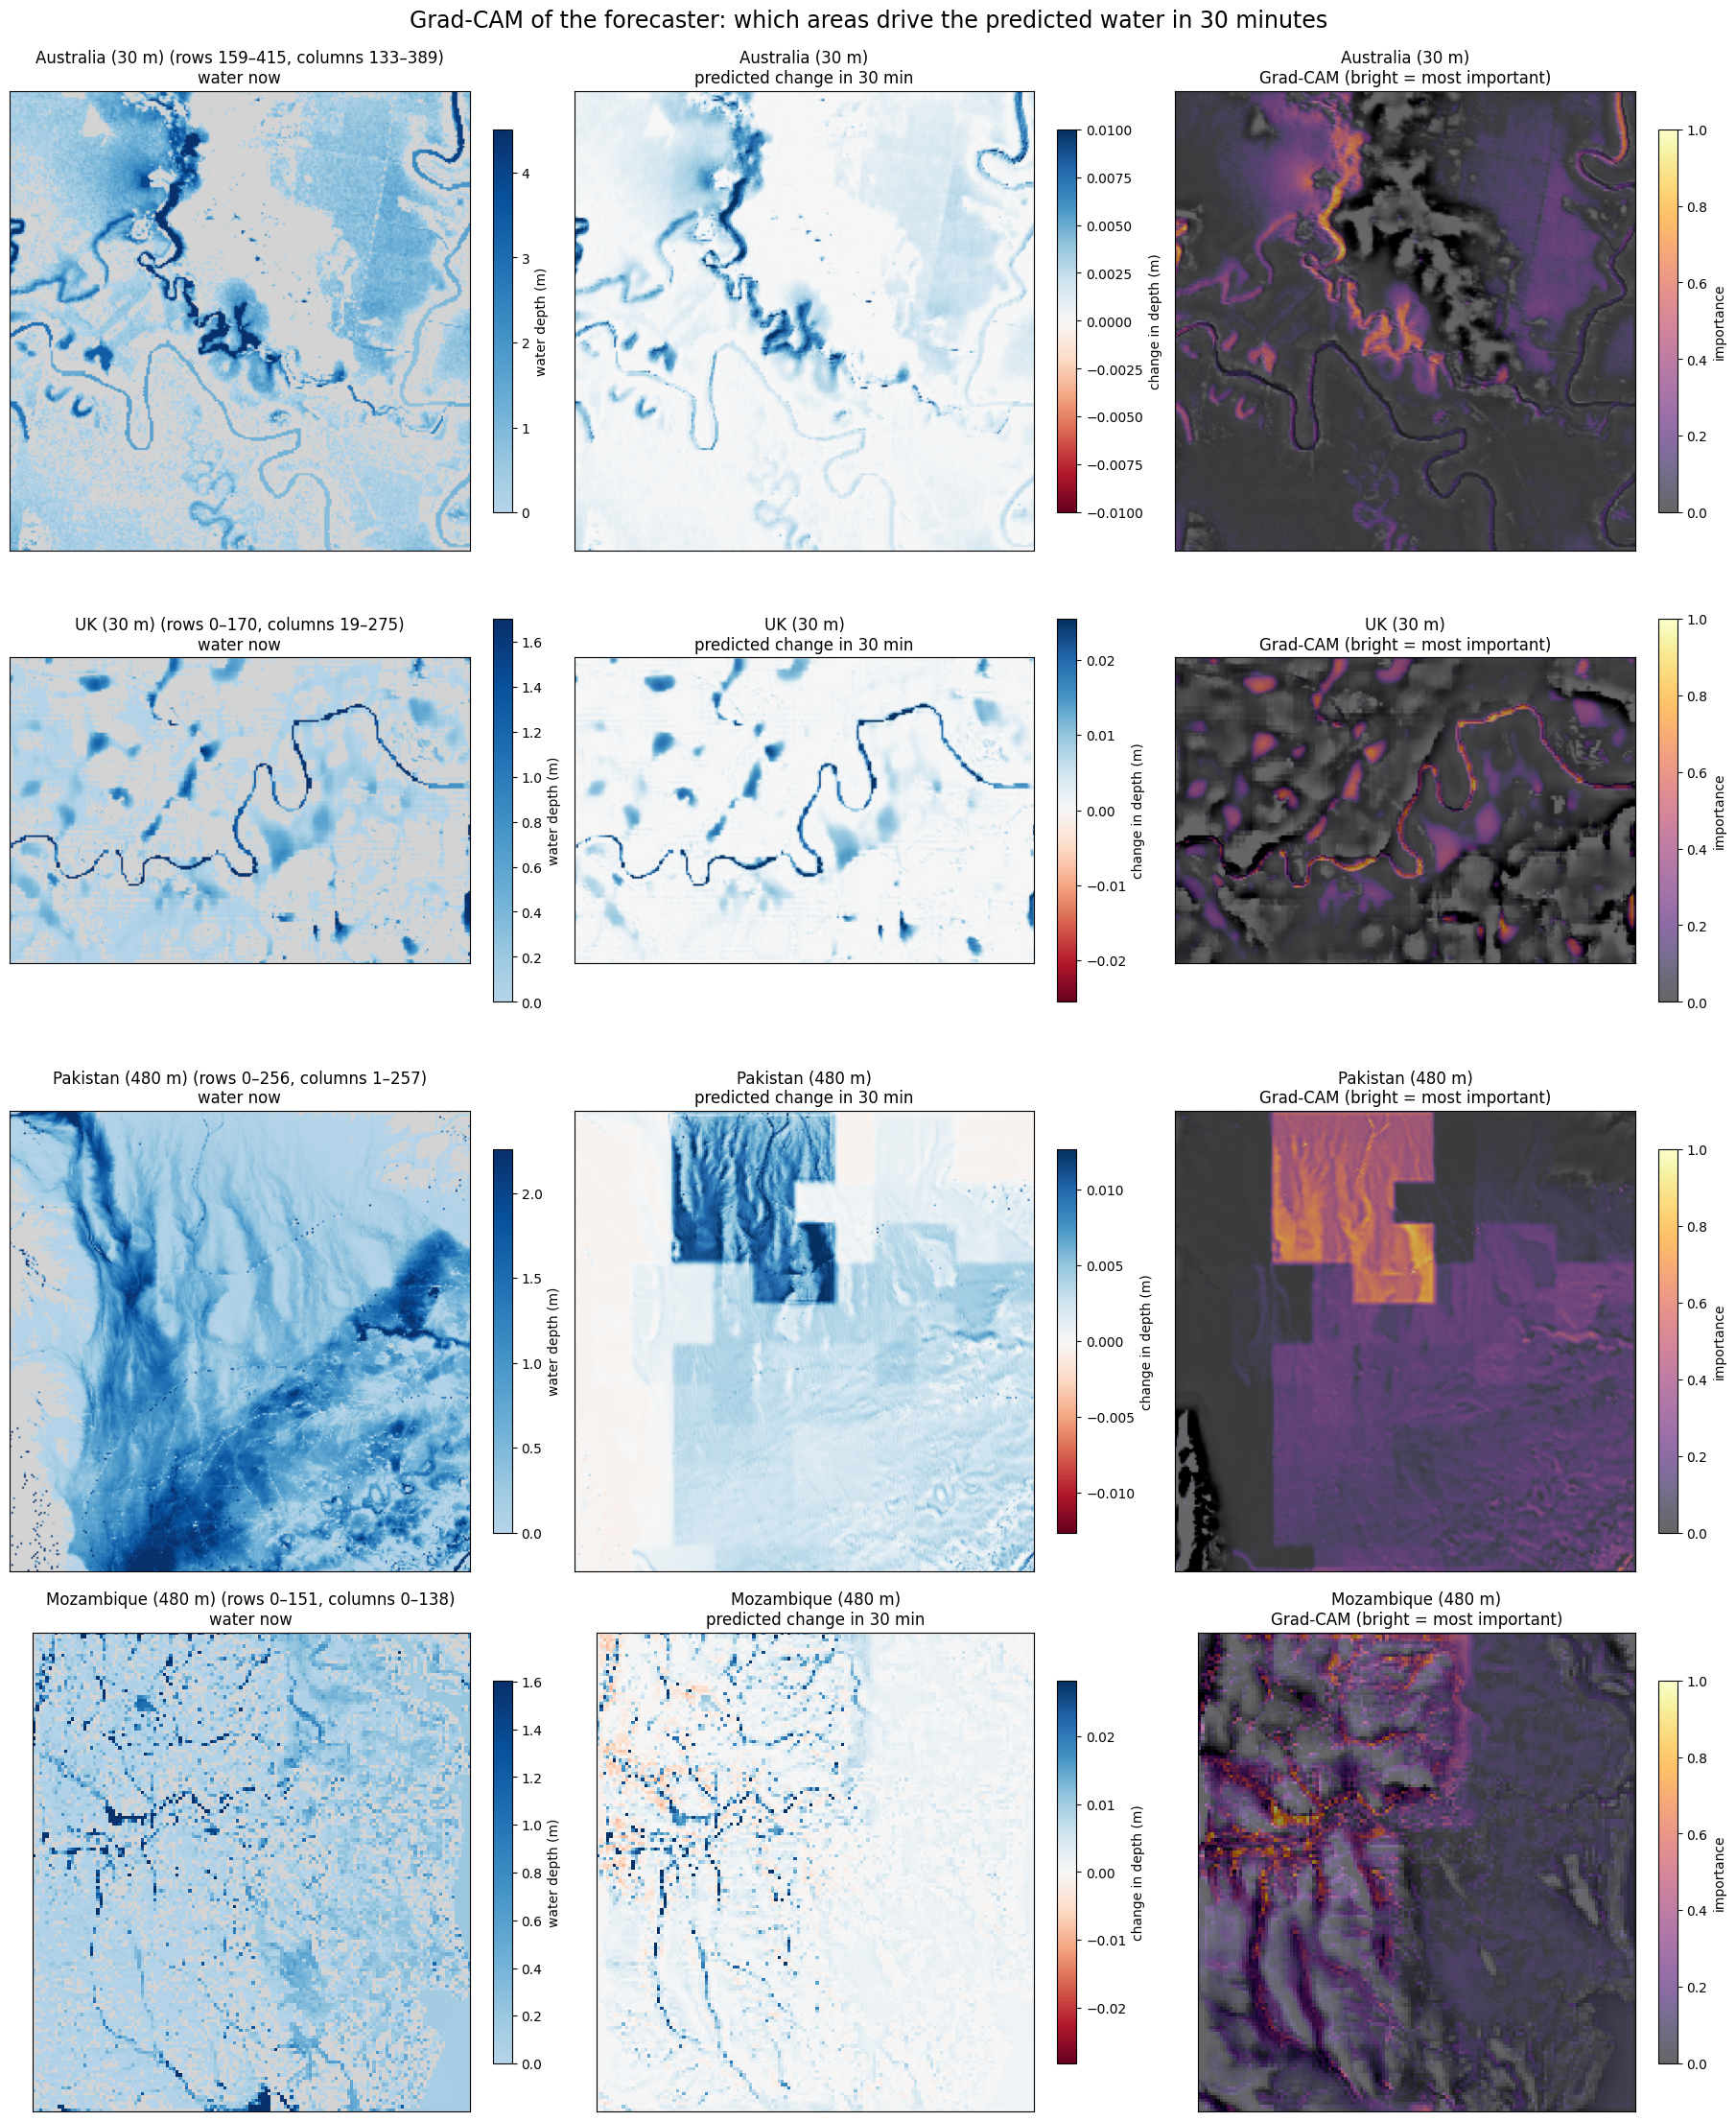
\includegraphics[width=\linewidth]{img/grad_cam_forecaster.png}\captionof{figure}{Grad-CAM of the forecaster (Model A): water now, predicted change, heat map over local ground height. \textbf{Say this:} the bright places follow rivers and flood edges.}
\end{minipage}\hfill
\begin{minipage}[t]{0.47\linewidth}\centering
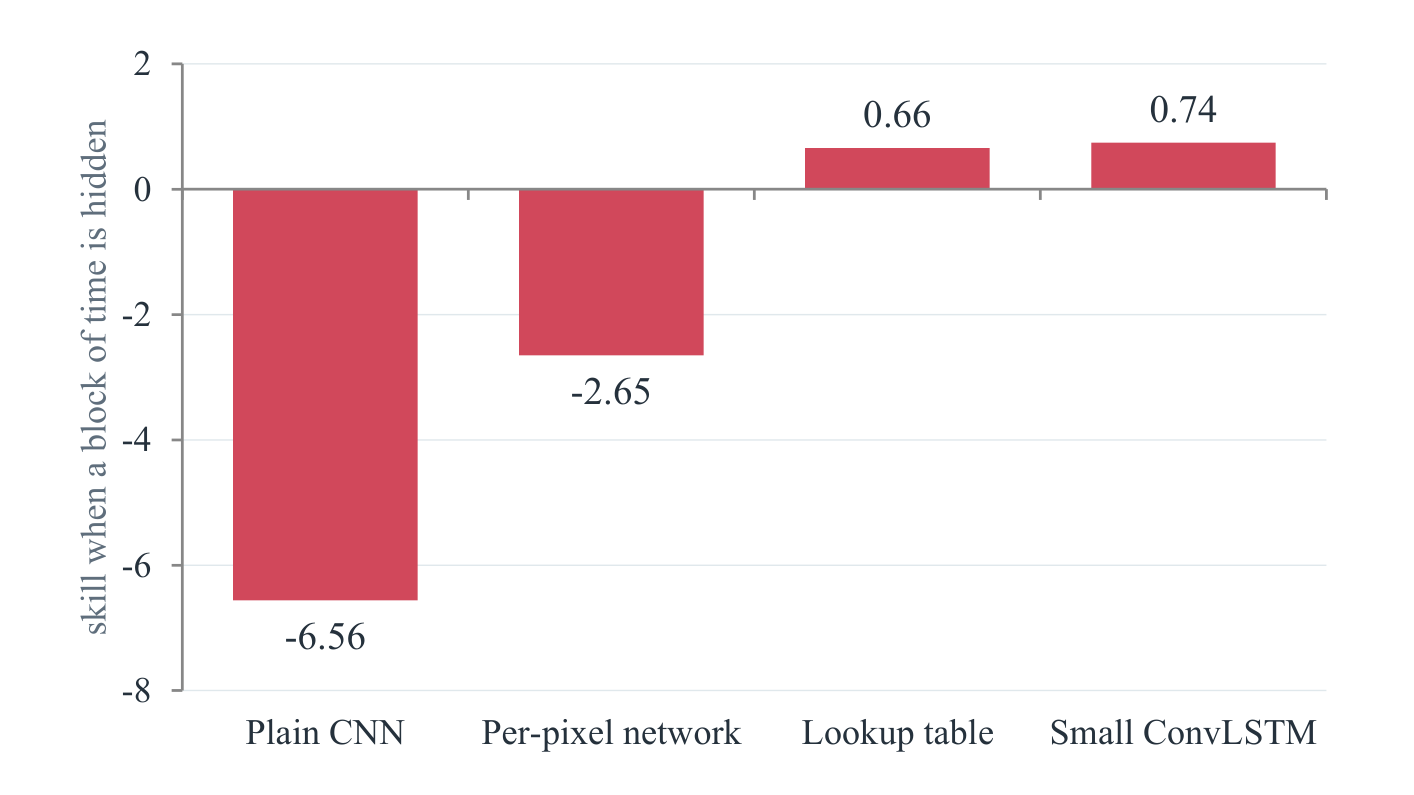
\includegraphics[width=\linewidth]{img/strict_split.png}\captionof{figure}{The strict test (start of a flood hidden). \textbf{Say this:} the plain CNN breaks down, the ConvLSTM and lookup table stay steady.}
\end{minipage}
\end{figure}

\textbf{Where each course keyword appears:} CNN (Chapters 5, 10), LSTM and ConvLSTM (6, 10, 13), capsule network (15), NeuroSymbolic AI (11, 15), explainable AI and Grad-CAM (16).

% =========================================================== CHAPTER 17
\section{Limits, lessons and what comes next}\label{ch:limits}

\textbf{What this study cannot tell you.} Only two independent test pairs (Australia to UK, Pakistan to Mozambique). The floods are simulated. Part 1 results are single runs. The two parts use different protocols and cannot be compared. The capsule network and Grad-CAM were built on Model A, not B. The LSTM memory is untested beyond 2.5 hours. A plain CNN can break completely at the start of a flood it never saw.

\textbf{Lessons.} (1) Compare every model with simple forecasts. (2) A weak baseline flatters a model. (3) Check your own explanations (we first thought Model A never saw draining water, and the data said no). (4) A bigger network is not automatically better. (5) Know your noise: differences below about 0.02 are not claimed. (6) Test on unseen places and hide a block of time too. (7) Write hypotheses down first, and say what you do not know.

\textbf{Next.} Forecast 6 to 24 hours by feeding forecasts back. Split Model B's two changes apart. Rebuild the capsule network and Grad-CAM on Model B. Repeat the Colab runs with several seeds.

\textbf{Conclusion.} We built a CNN-ConvLSTM forecaster for flood depth maps, added a capsule severity network, Grad-CAM and written rules, and tested them on later parts of the training floods and on floods from other countries. Model A beat the easiest reference and looked successful, a second simple reference was far better, and Model B matched it. The laptop study showed the depth history carries nearly all of the skill, and at equal training length the ConvLSTM was no more accurate than a plain CNN, though steadier when the start of a flood was hidden.

% =========================================================== KEY NUMBERS
\origsection{The key numbers on one page}\label{ch:nums}

Part 1 is the Colab notebook and Part 2 the laptop study. The four tests are always in the order Australia, UK, Pakistan, Mozambique.

\begin{table}[!htbp]
\centering\small
\caption{The numbers to remember.}
\begin{tabularx}{\linewidth}{|>{\bfseries}p{4.3cm}|Y|}
\hline
\rowcolor{black!12} \hd{What} & \hd{The number}\\ \hline
The floods & Four. Learn from Australia and Pakistan, test on the never-seen UK and Mozambique.\\ \hline
Square sizes & 30 m (Australia, UK) and 480 m (Pakistan, Mozambique).\\ \hline
Maps kept & One every 30 minutes: 481, 145, 673 and 289 maps.\\ \hline
Part 1 forecaster & 62,833 parameters. Four maps in, one map out, 30 minutes ahead.\\ \hline
Error of copying the last map & 0.112, 0.520, 0.103 and 0.548 cm.\\ \hline
Trend number $\beta$ & 0.921 for 30 m and 0.948 for 480 m.\\ \hline
Skill of the trend forecast & 0.990, 0.947, 0.908 and 0.942.\\ \hline
Skill of Model A & $-1.449$, 0.305, 0.345 and 0.150.\\ \hline
Skill of Model B & 0.989, 0.948, 0.908 and 0.943.\\ \hline
Error left after the trend & 1\%, 5\%, 9\% and 6\% of the error of copying.\\ \hline
Part 2 size & About 310 training runs. Five maps in, five out, up to 2.5 hours ahead.\\ \hline
Part 2 skill & Lookup table 0.74 to 0.79. Linear model 0.79 to 0.82. Best networks 0.81 to 0.87. Original CNN-LSTM 0.06 to 0.19.\\ \hline
Noise between seeds & 0.006 to 0.010, so treat differences below about 0.02 as noise.\\ \hline
A network 140 times larger & No gain (0.840 and 0.802).\\ \hline
Capsule network against a plain layer & 67.8\% against 60.2\%, but 80.3\% against 79.8\% with augmentation.\\ \hline
Capsule network with the rules (Part 1) & 67.9\%, 56.1\%, 89.1\% and 70.7\%.\\ \hline
Grad-CAM deletion test & 84\% to 92\% of windows for the depth forecast.\\ \hline
Strict test on hidden Pakistan tiles & Plain CNN 0.430 down to $-6.56$. ConvLSTM 0.742. Lookup table 0.66.\\ \hline
\end{tabularx}
\end{table}
